%------------------------------- CHAPTER NAME --------------------------------
\chapter{Payload-Range}

\begin{flushright}
	{\smaller
		\textit{All men dream: but not equally. Those who dream by night in the dusty recesses of their minds \\ wake in the day to find that it was vanity: but the dreamers of the day are dangerous men,\\ for they may act their dreams with open eyes, to make it possible. This I did.}\\
		-- T.E Lawrence "Lawrence of Arabia"}
\end{flushright}

\noindent
The Payload-Range diagram is a very important resource in aircrafts design because it allows to illustrate an aircraft operational limits by showing the trade-off relationship between the payload that can be carried and the range that can be flown; moreover, in synergy with the \gls{DOC} diagram, it is very useful to the future aircraft customers to have an idea of expected profits derived by their investment.
%
Payload-Range is also a key feature of the design requirements so it is possible to state that its relevance is felt through all the conceptual and preliminary design phases.
%
%-------------------------- THEORETICAL BACKGROUND ---------------------------
\section{Theoretical background}
To better understand the theoretical background behind this diagram, the first step is to focus the attention upon the link between the range and the fuel consumption, which is influenced by aircraft weight through Breguet formulas. 
%
It’s possible to imagine, at first, an aircraft in which payload and fuel weights can be managed at will, so that, in this completely flexible aircraft, the more the required range is, the less is the payload in order to carry more fuel at a specified maximum take-off weight; this leads to the diagram in figure~\ref{fig:Figure1}.
%
\begin{figure}[t] 
\centering
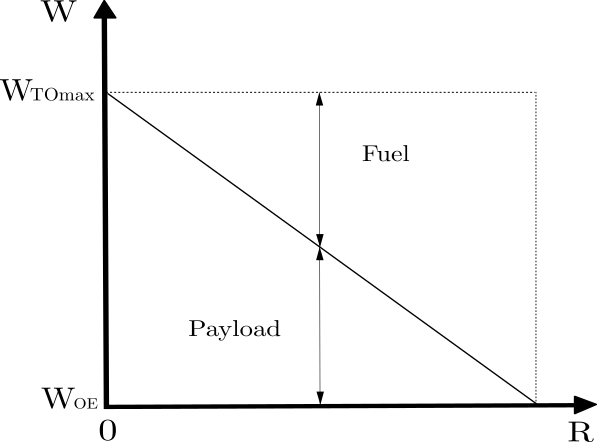
\includegraphics[keepaspectratio, width=0.6\textwidth]{Flexible_Payload_Range}
\caption{Payload-Range for a completely flexible aircraft}
\label{fig:Figure1}
\end{figure}
%
Because the payload is carried in the fuselage while the fuel is carried in wing tanks, the more the payload, the more the weight in the fuselage; this means that wings are incrementally more bending loaded so that a heavier structure is required. However, in this way the operating empty weight grows up limiting the payload the aircraft can carry, at that maximum take-off and fuel weights, for that range; the consequence of this is that, in particular for long range missions, the payload is too low, providing low profits.
%
In order to avoid this situation it is possible to decide, preventively, the maximum payload weight the aircraft can carry in fuselage so that the maximum bending load for wings and, in consequence their structural weight, is set; this particular weight is named \gls{acr:MZFW}. As a result of this, the previous diagram changes in the one reported in figure~\ref{fig:Figure2} which starts with the maximum zero fuel weight and keep it constant until the maximum take-off weight is reached. From this point on, the far the aircraft have to go, the more the fuel it needs, but, since the maximum take-off weight is set, the only way to increase fuel weight is to reduce the payload; this condition is represented by the second segment of the diagram and, along this, the aircraft weight is always equal to the maximum take-off weight. With further increase of the required range for the aircraft, the fuel tanks maximum capacity will be reached prevent to store more fuel; the only solution at this problem is to put the additional fuel into the fuselage, reducing, consequently, the payload weight in order to respect the maximum zero fuel weight limitation. Along this last segment the payload weight decreases more rapidly with increasing range reaching, ideally, the value of zero at which the flight mission is useless; moreover the aircraft weight is not equal to the maximum take-off weight anymore but to a lower one.

\bigskip
\begin{figure}[b]
\centering
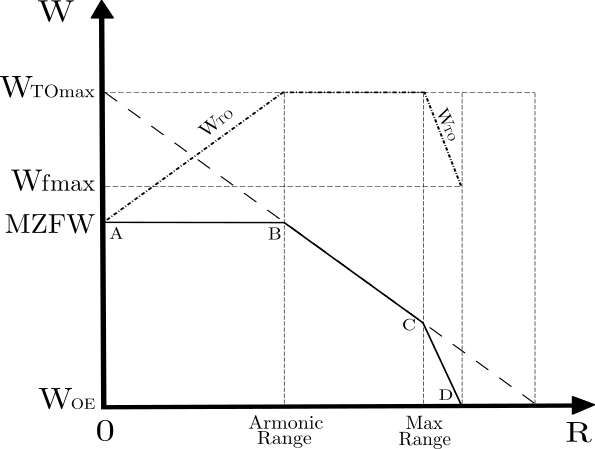
\includegraphics[keepaspectratio, width=0.6\textwidth]{Payload_Range}
\caption{Payload-Range with MZFW limitation}
\label{fig:Figure2}
\end{figure}

\bigskip
\noindent
Now that the theory behind the Payload-Range is explained, it is interesting to see how to build up the diagram. For this purpose at least the preliminary weight estimation has to be done in order to know the value of the following weights.
%
\begin{itemize}
\item W\textsubscript{TO}
\item W\textsubscript{OE}
\item W\textsubscript{Payload}
\end{itemize}
%
\noindent 
Furthermore four fundamental couples of payload and range values have to be defined:
%
\begin{itemize}
\item Point A, in which the payload is the maximum allowed and the range is zero.
\item Point B, in which the maximum range, with maximum take-off weight and maximum payload, is reached. This range value is called Harmonic Range.
\item Point C, in which the fuel tanks full capacity is reached with a payload lower than the maximum one and still the maximum take-off weight.
\item Point D, in which the take-off weight decreases because of the reduction of payload to zero in order to store more fuel in the fuselage.
\end{itemize}
%
\noindent
Since point A is very simple to obtain, it is more interesting to analyze how to calculate points B, C and D coordinates.
%
For point B it is necessary to focus the attention upon Breguet formulas in order to calculate the maximum range the aircraft can fly at maximum take-off weight with maximum payload; these are different for jet or propeller aircraft and can be written as follow, with the range R in \si{}{\km}, \gls{acr:SFC} in $\frac{\si{lb}}{\si{hp}\cdot\hour}$ and \gls{acr:SFCJ} in $\frac{\si{lb}}{\si{lb}\cdot\hour}$.
%
\begin{subequations}\label{eqn:BreguetEquation}
\begin{equation}\label{eqn:BreguetEquationProp}
R=
      \begin{array}{l@{\rule{2em}{0pt}}l} 
      603.5\cdot \left(\frac{\eta_{p}}{SFC}\right)_{\text{cruise}}\cdot \left(\frac{L}{D}\right)_{\text{cruise}}\cdot \ln\left(\frac{W_{i}}{W_{f}}\right)
          & \text{if} \;\, \text{propeller engine driven}
      \end{array}
\end{equation}
\begin{equation}\label{eqn:BreguetEquationJet}
R=
      \begin{array}{l@{\rule{7em}{0pt}}l} 
      \left(\frac{V}{SFCJ}\right)_{\text{cruise}}\cdot \left(\frac{L}{D}\right)_{\text{cruise}}\cdot \ln\left(\frac{W_{i}}{W_{f}}\right)
          & \text{if} \;\, \text{jet engine driven}
      \end{array}
\end{equation}
\end{subequations}

\noindent
Knowing the specific fuel consumption, the aerodynamic and propeller efficiency, or speed for jet aircraft, in cruise condition, the only unknown left for calculate the range is the weight ratio. In order to calculate this it is necessary to start by evaluating the amount of fuel the airplane can take on board, at maximum take-off weight and maximum payload, with the following formula.
%
\begin{equation}
W_{TO,\text{max}}=W_{OE}+W_{\text{payload,max}}+W_{\text{fuel}}
\label{eqn:Equation1.3}
\end{equation}

\noindent
Once the used fuel weight is known, it is possible to use the fuel fraction method from the weight estimation design phase in order to find the total weight ratio across the entire aircraft mission. 
%
\begin{equation}
W_{\text{fuel}}=\left(1-M_{ff}\right)\cdot W_{TO}
\label{eqn:Equation1.4}
\end{equation}

\noindent
$M_{ff}$ is the fuel fraction of the entire mission profile given by the following expression.

\bigskip
\begin{equation}
M_{ff}=\frac{W_1}{W_{TO}}\cdot 
	   \frac{W_2}{W_{1}}\cdot
	   \frac{W_3}{W_{2}}\cdot 
	   \frac{W_4}{W_{3}}\cdot 
	   \frac{W_5}{W_{4}}\cdot 
	   \frac{W_6}{W_{5}}\cdot 
	   \frac{W_7}{W_{6}}\cdot 
	   \frac{W_8}{W_{7}}\cdot 
	   \frac{W_9}{W_{8}}\cdot 
	   \frac{W_{10}}{W_{9}}\cdot 
	   \frac{W_{\text{final}}}{W_{10}} 
	   \label{eqn:Equation1.5} 
\end{equation}

\noindent
From this point on, it is necessary to have a table, like the one of table~\ref{table:Table1}, in which all weight ratios can be found statistically except for cruise, alternate cruise and loiter phases; these three unknown ratios are those that build up the Breguet weight ratio required by the range formula.   

\bigskip
\begin{table}[!ht]
\centering
\begin{tabular}{p{2.7cm}p{1.8cm}p{1.1cm}p{1.7cm}p{2.4cm}p{1.2cm}p{2.1cm}}
\toprule
\textbf{Airplane type} & \textbf{Start}, \textbf{Warm-up} & \textbf{Taxi} & \textbf{Take-off} & \textbf{Brief descent} & \textbf{Brief climb} & \textbf{Landing, Taxi and Shutdown} \\
\midrule
Homebuilts                     & 0,998 & 0,998 & 0,998 & 0,995 & 0,995 & 0,995       \\[0.7cm]
Single Engine                  & 0,995 & 0,997 & 0,998 & 0,992 & 0,993 & 0,993       \\[0.7cm]
Twin Engine                    & 0,992 & 0,996 & 0,996 & 0,990 & 0,992 & 0,992       \\[0.7cm]
Agricultural                   & 0,996 & 0,995 & 0,996 & 0,998 & 0,999 & 0,998       \\[0.7cm]
Business Jets                  & 0,990 & 0,995 & 0,995 & 0,980 & 0,990 & 0,992       \\[0.7cm]
Regional TBP's                 & 0,990 & 0,995 & 0,995 & 0,985 & 0,985 & 0,995       \\[0.7cm]
Transport Jets                 & 0,990 & 0,990 & 0,995 & 0,980 & 0,990 & 0,992       \\[0.7cm]
Mil. Trainers                  & 0,990 & 0,990 & 0,990 & 0,980 & 0,990 & 0,995       \\[0.7cm]
Fighters                       & 0,990 & 0,990 & 0,990 & 0,960-0,900 & 0,990 & 0,995     \\[0.7cm]
Mil.Patrol,Bmb and Trspt       & 0,990 & 0,990 & 0,995 & 0,980 & 0,990 & 0,992       \\[0.7cm]
Flying boats,Amph. and Floats  & 0,992 & 0,990 & 0,996 & 0,985 & 0,990 & 0,990       \\[1.2	cm]
Supersonic Cruise              & 0,990 & 0,995 & 0,995 & 0,920-0,870 & 0,985 & 0,992     \\[0.1	cm]
\bottomrule
\end{tabular}
\caption{Suggested fuel fractions}
\label{table:Table1}
\end{table}
%
\noindent
For the evaluation of point C, similar steps have to be followed with the difference that, in this case, the fuel is the maximum that the wing tanks can store and the payload is the unknown of the (\ref{eqn:Equation1.6}).
%
\begin{equation}
W_{TO,\text{max}}=W_{OE}+W_{\text{payload}}+W_{\text{fuel,max}}
\label{eqn:Equation1.6}
\end{equation}

\noindent
From this equation it is possible to calculate point C ordinate, while for the range abscissa the same procedure used for point B range has to be followed with the difference that now it is necessary to use the fuel weight relative to the maximum fuel tank capacity which is known from the wing fuel tank design.
%
Finally for point D, the payload is set at zero so that is possible to evaluate the $W_{\text{TO}}$, relative to maximum fuel weight with no passengers, from the following equation.
%
\begin{equation}
W_{\text{TO}}=W_{\text{OE}}+W_{\text{fuel,max}}
\label{eqn:Equation1.7}
\end{equation}
%
\noindent
This new take-off weight generates a lower $M_{ff}$, from fuel fraction equation, which leads to a bigger weight ratio to be used in Breguet formulas with the result of a bigger range.
%
%------------------------- JAVA CLASS ARCHITECTURE ---------------------------
\section{Java class architecture}
In this paragraph the implementation in the \gls{JPAD} software of the Payload-Range diagram, through the \lstinline[language=Java]!PayloadRangeCalc! Java class, is presented. The idea has been to create a dedicated Java class which is demanded of the calculation of the four couple of range and payload values presented before; moreover it has to confront the user chosen Mach number condition with the best range one and to parametrize the analysis at different maximum take-off weight in order to help users making design decisions about different version of the same aircraft.
%
The class core consists of the following three principal methods which have to evaluate points B, C and D coordinates using the procedure explained before.
%
\begin{itemize}
\item\lstinline[language=Java]!calcRangeAtMaxPayload!
\item\lstinline[language=Java]!calcRangeAtMaxFuel!
\item\lstinline[language=Java]!calcRangeAtZeroPayload!
\end{itemize}
%
\noindent
Each of these requires in input the table~\ref{table:Table2} data, a database which collects all data from table~\ref{table:Table1},  named \lstinline[language=Java]!FuelFractionDatabaseReader!, and an engine database, for turboprop or turbofan, in which all specific fuel consumption values, at given Mach number and altitude, are stored.
%
\begin{table}[!ht]
\begin{tabular}{p{7cm}p{7.5cm}}
\toprule
\lstinline[language=Java]!maxTakeOffMass! & Maximum take-off mass \\[0.1	cm]
\lstinline[language=Java]!sweepHalfChordEquivalent! & Equivalent wing sweep angle at half chord \\[0.1cm]
\lstinline[language=Java]!surface! & Wing surface \\[0.1cm]
\lstinline[language=Java]!cd0!	& Wing c\textsubscript{D0} \\[0.1cm]
\lstinline[language=Java]!oswald!	& Wing Oswald factor \\[0.1cm]
\lstinline[language=Java]!cl!	& The current lift coefficient in cruise configuration \\[0.1cm]
\lstinline[language=Java]!ar!	& Wing aspect ratio \\[0.1cm]
\lstinline[language=Java]!tcMax! & Mean maximum thickness of the wing \\[0.1cm]
\lstinline[language=Java]!byPassRatio! & Engine by-pass ratio (when needed) \\[0.1cm]
\lstinline[language=Java]!eta! & Propeller efficiency (when needed) \\[0.1cm]
\lstinline[language=Java]!altitude! & Cruise altitude \\[0.1cm]
\lstinline[language=Java]!currentMach! & The actual Mach number during cruise \\[0.1cm]
\lstinline[language=Java]!isBestRange! & A boolean variable that is true if the evaluation of the best range condition is performed, otherwise it's false         \\
\bottomrule
\end{tabular}
\caption{Input data}
\label{table:Table2}
\end{table}
%
From this point on, the evaluation of (\ref{eqn:Equation1.3}), (\ref{eqn:Equation1.6}) and (\ref{eqn:Equation1.7}), for each method, and of (\ref{eqn:Equation1.4}), for all of them, is performed in order to set up the following calculations and to obtain the unknown value of the payload in point~C case; after that the fuel fractions database is read in order to obtain all known data necessary to calculate the required weight ratio to be used in (\ref{eqn:BreguetEquationProp}) or (\ref{eqn:BreguetEquationJet}) depending on the aircraft engine type. It is important to highlight that the database reading process is made up so that it can recognize all different kind of aircraft from table~\ref{table:Table1} and read the related line values.

\bigskip
\noindent
Since each method has to compare the chosen Mach number condition with the best range one, the boolean variable presented before is used in order to distinguish between different application cases; in this way, when the user specify the aircraft engine type and the boolean variable, the method reads the specific fuel consumption value, at given Mach number and altitude, from the related engine database and performs the calculation of the lift and drag wing coefficients which are then used to obtain the aerodynamic efficiency value. At this point is possible to calculate the range that represents point B, C or D abscissa. 
%
It should be noted that, in case of a true value of the boolean variable, the evaluation of the lift and drag wing coefficients, as well as the best range Mach number that replaces the user chosen one, is performed by calculating the parabolic drag polar characteristic points and choosing those that maximizes the range (point E for the turboprop and point A for the turbofan); whereas for a false value of the boolean variable, the lift coefficient is calculated by using the current flight condition angle of attack into the linear part of the wing lift curve, while the drag coefficient is evaluated from the aircraft total drag polar taking also into account potential wave drag sources.   

\bigskip
\noindent
Now that all points coordinates are known, the two following methods are demanded to build up abscissas and ordinates values arrays to be used in plotting the diagram.
%
\begin{itemize}
\item\lstinline[language=Java]!createRangeArray!
\item\lstinline[language=Java]!createPayloadArray!
\end{itemize}
%
\begin{table}[!ht]
\centering
\makebox[\textwidth]{
\begin{tabular}{cc}
\toprule
\textbf{Range Array} & \textbf{Payload Array} \\ 
\midrule
0,0	& Maximum payload, in number of passengers \\ [0.2cm]
\lstinline[language=Java]!calcRangeAtMaxPayload! output &	Maximum payload, in number of passengers \\ [0.2cm]
\lstinline[language=Java]!calcRangeAtMaxFuel! output &	Payload calculated in \lstinline[language=Java]!calcRangeAtMaxFuel! \\ [0.2cm]
\lstinline[language=Java]!calcRangeAtZeroPayload! output &	0,0 \\ [0.2cm]
\bottomrule
\end{tabular}
}
\caption{Payload and range array components}
\label{table:Table3}
\end{table}
%
\noindent
They use the Java \gls{List} interface to generate an ordered collection of values which are then populated with the following values.

\bigskip
\noindent
Finally the two arrays are used as input, together with another one from the best range condition analysis, for the last method, named~\lstinline[language=Java]!createPayloadRangeCharts_Mach!, that has to plot the diagram; this uses the~\lstinline[language=Java]!JFreeChart! Java library\cite{jfreechart} to generate a \gls{PNG} output image into the output folder of the software and is also able to create a \gls{TiKZ} version of the diagram to be used in \LaTeX.
%
As said before, this class finds another purpose in parameterizing the diagram in different maximum take-off weight conditions. To do that, the three core methods are used again inside a new one, named \lstinline[language=Java]!createPayloadRangeMatrices!, which implements a recursive calculation of the three points coordinates at different maximum take-off mass conditions generated by decreasing the original mass by 5$\%$ until it reaches a total decrease of 20$\%$. This new method requires the same input data reported in table~\ref{table:Table2} except for the maximum take-off mass which is generated inside the method itself. The output matrices are then used in a plotting method, equivalent to previous one but named \lstinline[language=Java]!createPayloadRangeCharts_MaxTakeOffMass!, which generates the \gls{PNG} and \gls{TiKZ} output images by receiving as input two matrices and not two arrays as before.

\bigskip
\begin{figure}[H]
\centering
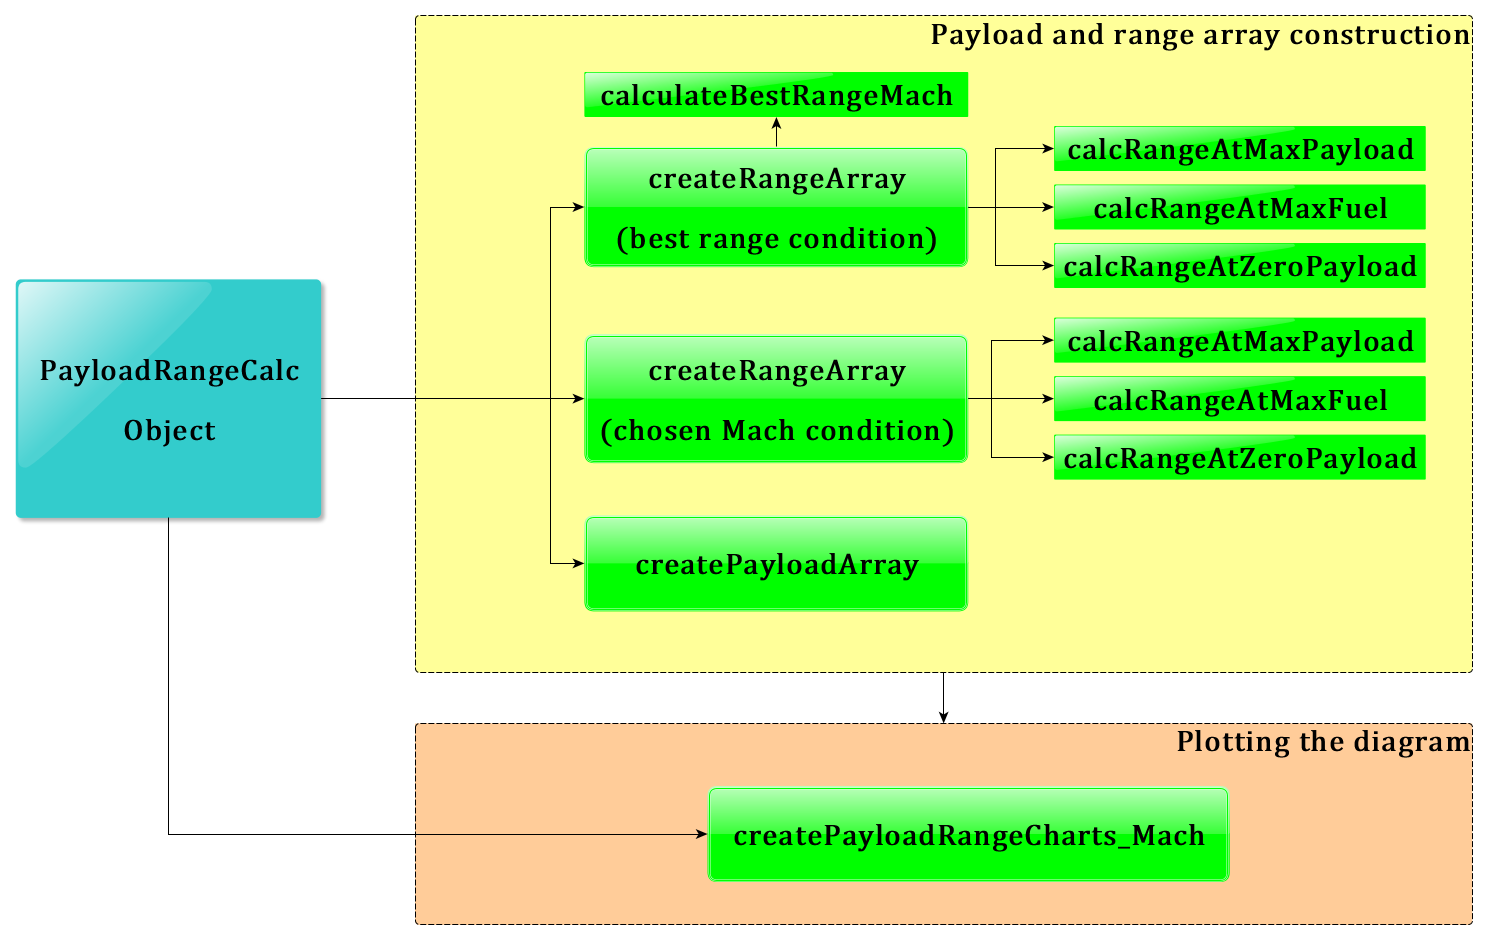
\includegraphics[keepaspectratio, width=0.83\textwidth]{PayloadRange_BestRange_Flowchart}
\caption{Payload-Range Java class flowchart for best range and chosen Mach conditions comparison}
\label{fig:Figure3}
\end{figure}

\bigskip
\begin{figure}[H]
\centering
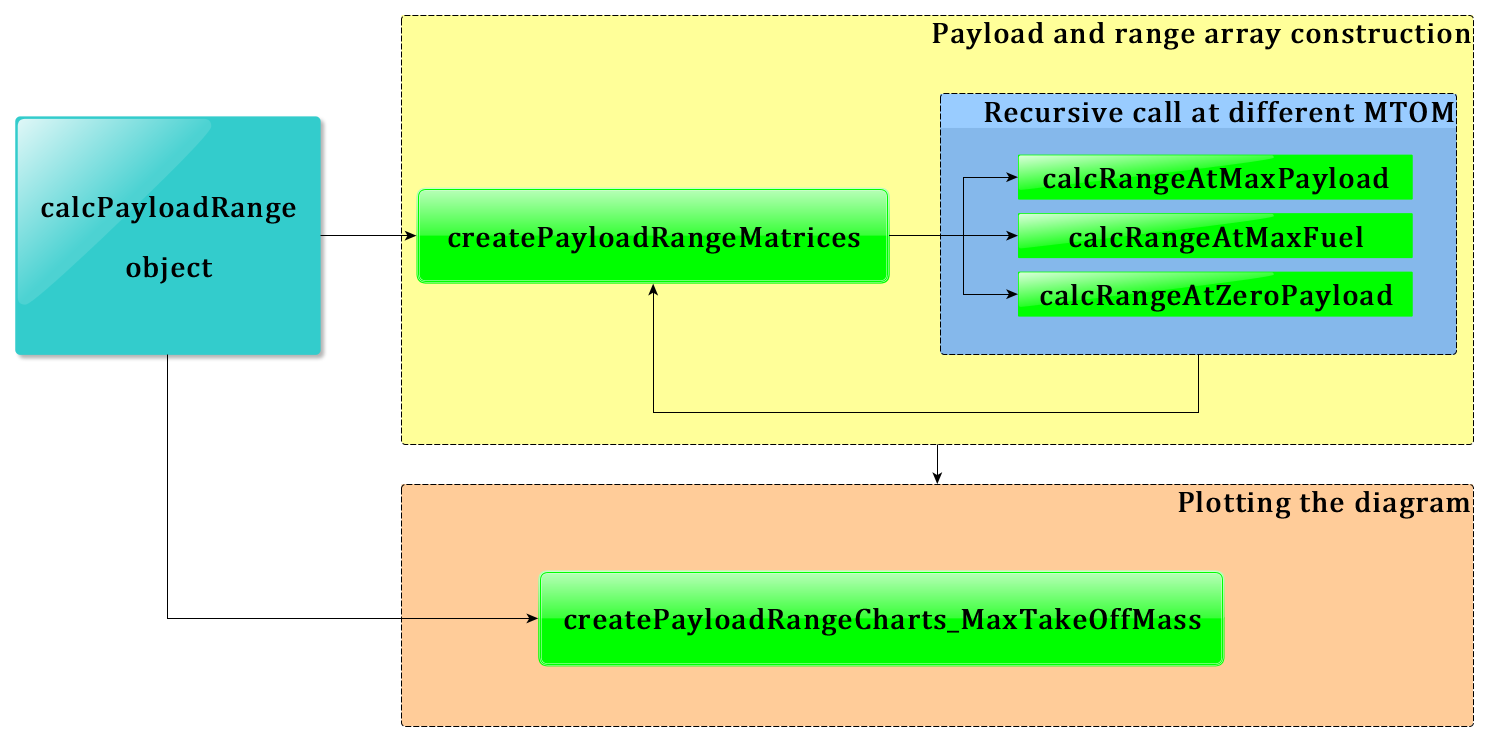
\includegraphics[keepaspectratio, width=0.83\textwidth]{PayloadRange_MTOM_Flowchart}
\caption{Payload-Range Java class flowchart for maximum take-off mass parameterization}
\label{fig:Figure4}
\end{figure}
%
%----------------------- CASE STUDY : ATR72 AND B747 -------------------------
%
\section{Case study: ATR-72 and B747-100B}
With the purpose of validating calculations presented before, two case studies have been taken into account; the first one is on the ATR-72 and the second one on the B747-100B.

\bigskip
\noindent
The two presented tests share the same architecture so that a general guideline can be followed; this strategy has been designed with the purpose of making a general procedure in order to simplify user work. Thus, for more clarity, the listings of test is reported, as an 	exemplifying practice, only in the case of the ATR-72. 

\bigskip
\noindent
The preliminary steps required to build up the test class are the same that have been discussed in the paragraph \ref{par:DefaultAircraft}. However, since the class \lstinline[language=Java]!PayloadRangeCalc! requires that data from table \ref{table:Table1} are available, another database has to be read. This database is named \lstinline[language=Java]!FuelFraction.h5! and is read by the class \lstinline[language=Java]!FuelFractionDatabaseReader! created following the guideline of appendix~\ref{par:Appendix2}.
%
Furthermore, this database is strictly connected with the fuel tank so that it has been decided to link the object of the class \lstinline[language=Java]!FuelFractionDatabaseReader! to this aircraft component as follows.

\bigskip
\begin{lstlisting}[caption={Attachment of the \lstinline!FuelFractionDatabaseReader! to the fuel tank component of the aircraft}, captionpos=b, tabsize=2]
		aircraft.get_theFuelTank().setFuelFractionDatabase(fuelFractionReader);
\end{lstlisting}
%
At this point all data required by the \lstinline[language=Java]!PayloadRangeCalc! class are now ready to be used and it’s possible to create an object of this class accessing, in this way, to all its methods, which have been explained in the previous paragraph. 

\bigskip
\begin{lstlisting}[caption={Excerpt of the ATR-72 Payload-Range test - Payload-Range class instance creation}, captionpos=b, tabsize=2]
		// Creating the Calculator Object
		PayloadRangeCalc test = new PayloadRangeCalc(
								theCondition, 
								aircraft,
								AirplaneType.TURBOPROP_REGIONAL
								);
\end{lstlisting}

\bigskip
\noindent
The first check that is implemented has the purpose of inspect whether or not the chosen cruise Mach number is bigger than the crest critical one; in this case a warning message is launched in order to inform the user of the situation. The method demanded of this is \lstinline[language=Java]!checkCriticalMach! which accepts in input a given Mach number, compares it with the one calculated with Kroo method~\cite{Ciornei:CriticalMach}, starting from the cruise lift coefficient, and return a boolean variable that is true only if the chosen Mach number is bigger than the crest critical one indeed. 

\bigskip
\begin{lstlisting}[caption={Excerpt of the ATR-72 Payload-Range test - critical Mach number check}, captionpos=b, tabsize=2]
		// ----------CRITICAL MACH NUMBER CHECK--------------
		boolean check = test.checkCriticalMach(theCondition.get_machCurrent()	);
		if (check)
			System.out.println("\n\n-------------------------"
			+"\nCurrent Mach lower then critical Mach number"
			+"\nCurrent Mach = " + theCondition.get_machCurrent() 
			+"\nCritical Mach = " + test.getCriticalMach() 
			+"\n\n\t CHECK PASSED -> PROCEDING TO CALCULATION "
			+"\n\n"
			+"-----------------------------------------------");
		else{
			System.err.println("\n\n-------------------------"
			+"\nCurrent Mach bigger then critical Mach number"
			+"\nCurrent Mach = " + theCondition.get_machCurrent() 
			+"\nCritical Mach = " + test.getCriticalMach() 
			+"\n\n\t CHECK NOT PASSED -> WARNING!!! "
			+"\n\n"
			+"--------------------------------------");
		}
\end{lstlisting}

\bigskip
\begin{lstlisting}[caption={Excerpt of the ATR-72 Payload-Range test results - critical Mach number check}, captionpos=b, tabsize=2]
Current Mach is lower then critical Mach number.
Current Mach = 0.43
Critical Mach = 0.6659791543529567
	 CHECK PASSED --> PROCEEDING TO CALCULATION 
\end{lstlisting}

\bigskip
\begin{lstlisting}[caption={Excerpt of the B747-100B Payload-Range test results - critical Mach number check}, captionpos=b, tabsize=2]
Current Mach is lower then critical Mach number.
Current Mach = 0.84
Critical Mach = 0.8490814607347361
	 CHECK PASSED --> PROCEEDING TO CALCULATION 
\end{lstlisting}

\bigskip
\noindent
At this point, if the user wants to compare the chosen Mach number condition with the best range one, all that it’s needed is to invoke the \lstinline[language=Java]!createRangeArray! method, for both the operative conditions, and the \lstinline[language=Java]!createPayloadArray! one; after that the diagram is generated from the method \lstinline[language=Java]!createPayloadRangeCharts_Mach!.

\bigskip
\begin{lstlisting}[caption={Excerpt of the ATR-72 Payload-Range test - Payload-Range diagram evaluation and plot}, captionpos=b, tabsize=2]
		// ----------------BEST RANGE CASE-------------------
		System.out.println("-------BEST RANGE CASE--------");
		List<Amount<Length>> vRange_BR = test
						.createRangeArray(
										test.getMaxTakeOffMass(),
										test.getSweepHalfChordEquivalent(),
										test.getSurface(),
										test.getCd0(),
										test.getOswald(),
										aircraft.get_theAerodynamics().getcLE(),
										test.getAr(),
										test.getTcMax(),
										test.setByPassRatio(0.0),
										test.getEta(),
										test.getAltitude(),
										test.calculateBestRangeMach(
														EngineTypeEnum.TURBOPROP,
														test.getSurface(),
														test.getAr(),
														test.getOswald(),
														test.getCd0(),
														test.getAltitude()),
										true);		
		// -------------USER CURRENT MACH-------------------
		System.out.println("------CURRENT MACH CASE-------");
		List<Amount<Length>> vRange_CM = test
						.createRangeArray(
										test.getMaxTakeOffMass(),
										test.getSweepHalfChordEquivalent(),
										test.getSurface(),
										test.getCd0(),
										test.getOswald(),
										test.getCl(),
										test.getAr(),
										test.getTcMax(),
										test.setByPassRatio(0.0),
										test.getEta(),
										test.getAltitude(),
										test.getCurrentMach(),
										false);
		// -------------------PLOTTING----------------------	
		// Mach parameterization:
		List<Double> vPayload = test.createPayloadArray();
		test.createPayloadRangeCharts_Mach(
						vRange_BR,
						vRange_CM,
						vPayload,
						test.calculateBestRangeMach(
										EngineTypeEnum.TURBOPROP,
										test.getSurface(),
										test.getAr(),
										test.getOswald(),
										test.getCd0(),
										test.getAltitude()),
						test.getCurrentMach());
\end{lstlisting}
%
\noindent
Otherwise, if it is the maximum take-off mass parameterization the wanted analysis, the required call is for \lstinline[language=Java]!createPayloadRangeMatrices! method followed by the plotting method \lstinline[language=Java]!createPayloadRangeCharts_MaxTakeOffMass!. 

\bigskip
\begin{lstlisting}[caption={Excerpt of the ATR-72 Payload-Range test - maximum take-off mass parameterization}, captionpos=b, tabsize=2]
		// -----------------MTOM PARAMETERIZATION----------
		test.createPayloadRangeMatrices(
						test.getSweepHalfChordEquivalent(),
						test.getSurface(),
						test.getCd0(),
						test.getOswald(),
						test.getCl(),
						test.getAr(),
						test.getTcMax(),
						test.setByPassRatio(0.0),
						test.getEta(),
						test.getAltitude(),
						test.getCurrentMach(),
						false
						);
		// ------------------PLOTTING----------------------		
		// MTOM parameterization:
		test.createPayloadRangeCharts_MaxTakeOffMass(
						test.getRangeMatrix(),
						test.getPayloadMatrix()
						);
\end{lstlisting}

\bigskip
\noindent
In conclusion, following pages shows a summary of input data used for each analyzed aircraft, together with their related results in terms of Payload-Range diagrams for both the chosen Mach number and best range comparison and max take-off mass parameterization. 
%
\begin{table}[H]
\makebox[\linewidth]{
\begin{minipage}{6cm}
\leftline{	
\begin{tabular}{cc}
\toprule
\textbf{Variables} & \textbf{Values} \\
\midrule
Range (point A) & 0 nmi \\
Payload (point A) & 72 passengers \\
\midrule
Range (point B) & 547.310 nmi \\
Payload (point B) & 72 passengers \\
\midrule
Range (point C) & 1357.730 nmi \\
Payload (point C) & 52 passengers \\
\midrule
Range (point D) & 1994.0560 nmi \\
Payload (point D) & 0 passengers \\
\midrule
$C_L$ & 0.421 \\
$C_D$ & 0.0356 \\
SFC & 0.424 \\
\bottomrule
\end{tabular}
}
\end{minipage}
\hspace{2.5cm}
\begin{minipage}{6cm}
\rightline{
\begin{tabular}{cc}
\toprule
\textbf{Variables} & \textbf{Values} \\
\midrule
Range (point A) & 0 nmi \\
Payload (point A) & 550 passengers \\
\midrule
Range (point B) & 4993.586 nmi \\
Payload (point B) & 550 passengers \\
\midrule
Range (point C) & 4995.0144 nmi \\
Payload (point C) & 550 passengers \\
\midrule
Range (point D) & 6454.205 nmi \\
Payload (point D) & 0 passengers \\
\midrule
$C_L$ &0.385 \\
$C_D$ & 0.0277 \\
SFC & 0.633 \\
\bottomrule
\end{tabular}
}
\end{minipage}
}
\caption{Review of ATR-72 (left) and B747-100B (right) results at chosen Mach number conditions}
\label{table:Table6}
\end{table}
%
\begin{table}[H]
\makebox[\linewidth]{
\begin{tabular}{llllll}
\toprule
\textbf{ } & \textbf{ATR-72} &\textbf{ } &  \textbf{JPAD} &\textbf{ } & \textbf{Difference(\%)}\\
\midrule
\textbf{Range} & 890 nmi  & \textbf{ } &$\approx820$ nmi &\textbf{ } & $\approx7.865$\%\\
\textbf{Payload} & 68 pass. at $\SI{95}{\kilogram}$ &\textbf{ } & 65 pass. at $\SI{99}{\kilogram}$ &\textbf{ } & \textbf{ }\\
\midrule
\textbf{ } & \textbf{B747-100B} &\textbf{ } & \textbf{JPAD} &\textbf{ } & \textbf{Difference(\%)} \\
\midrule
\textbf{Range} & $\approx5000$ nmi &\textbf{ } & 4714.5 nmi &\textbf{ } & $\approx5.71$\%\\
\textbf{Payload} & 452 pass. at $\SI{95}{\kilogram}$ &\textbf{ } & 550 pass. at $\SI{99}{\kilogram}$ &\textbf{ } & \textbf{ }\\
\bottomrule
\end{tabular}
}
\caption{Method results comparison with known data}
\end{table}
%
\begin{figure}[!t]
\centering
%PayloadRange_Mach
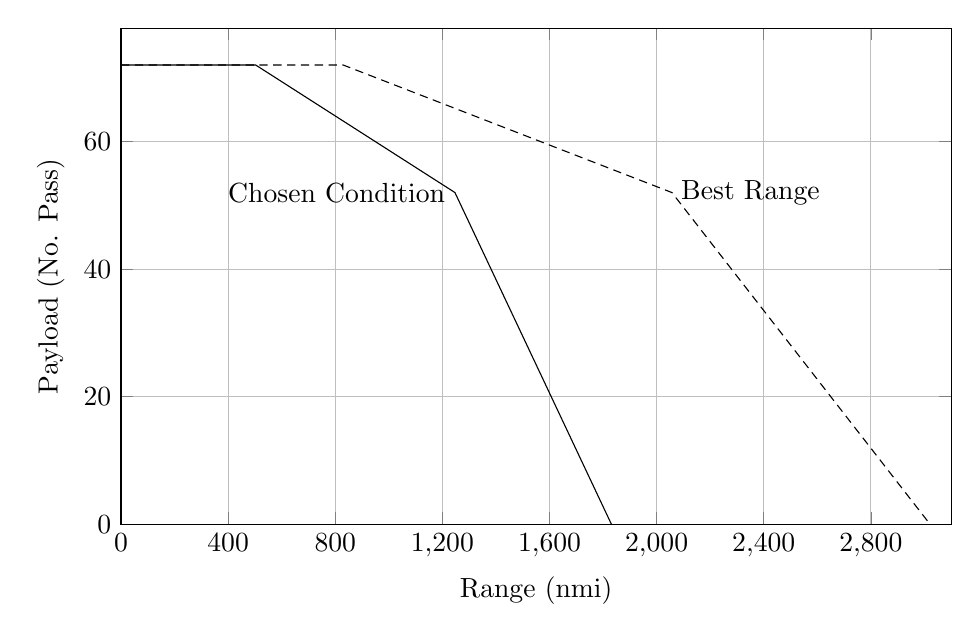
\begin{tikzpicture}

\begin{axis}[
%width=\figurewidth,
%height=\figureheight,
width=\textwidth,
height=0.65\textwidth,
scaled ticks=false, tick label style={/pgf/number format/fixed},
/pgfplots/xtick={0,400,...,3200},
xmin=0.0,
xmax=3100.0,
xlabel={Range (nmi)},
xmajorgrids,
ymin=0.0,
ymax=77.76,
ylabel={Payload (No. Pass)},
ymajorgrids,
legend style={at={(1.03,0.5)},anchor=west,draw=black,fill=white,legend cell align=left}
]

\addplot [
color=black,
densely dashed
]
table[row sep=crcr]{
0.0	72.0\\
829.1553643712685	72.0\\
2056.9859351535097	52.0\\
3021.021826278212	0.0\\
}node[right,pos=0.68] {Best Range};

\addplot [
color=black,
solid
]
table[row sep=crcr]{
0.0	72.0\\
502.58657991049535	72.0\\
1246.8272780900518	52.0\\
1831.1707223355413	0.0\\
}node[left,pos=0.68] {Chosen Condition};
\end{axis}
\end{tikzpicture}%

\caption{ATR-72 Payload-Range - Chosen Mach number and best range comparison}
\end{figure}
%
\begin{figure}[!b]
\centering
%PayloadRange_MaxTakeOffMass
\begin{tikzpicture}

\begin{axis}[
%width=\figurewidth,
%height=\figureheight,
width=\textwidth,
height=0.65\textwidth,
scaled ticks=false, tick label style={/pgf/number format/fixed},
xmin=0.0,
xmax=1977.6643801223847,
xlabel={Range (nmi)},
xmajorgrids,
ymin=0.0,
ymax=77.76,
ylabel={Payload (No. Pass)},
ymajorgrids,
%legend style={at={(1.03,0.5)},anchor=west,draw=black,fill=white,legend cell align=left}
legend entries = {$\SI{18500}{\kilogram}$\\$\SI{19600}{\kilogram}$\\$\SI{20800}{\kilogram}$\\$\SI{21900}{\kilogram}$\\$\SI{23100}{\kilogram}$\\},
]

\addplot [
color=black,
dotted
]
table[row sep=crcr]{
0.0	72.0\\
-1078.9286571061161	72.0\\
1755.07333490137	5.0\\
1831.1707223355413	0.0\\
};

\addplot [
color=black,
dashed
]
table[row sep=crcr]{
0.0	72.0\\
-649.2556391032156	72.0\\
1601.7689730994862	17.0\\
1831.1707223355413	0.0\\
};

\addplot [
color=black,
dashdotted
]
table[row sep=crcr]{
0.0	72.0\\
-244.14914205597876	72.0\\
1468.2276865740514	29.0\\
1831.1707223355413	0.0\\
};

\addplot [
color=black,
densely dashed
]
table[row sep=crcr]{
0.0	72.0\\
139.04873105524126	72.0\\
1350.839532297808	40.0\\
1831.1707223355413	0.0\\
};

\addplot [
color=black,
solid
]
table[row sep=crcr]{
0.0	72.0\\
502.58657991049535	72.0\\
1246.8272780900518	52.0\\
1831.1707223355413	0.0\\
};
\end{axis}
\end{tikzpicture}%

\caption{ATR-72 Payload-Range - Maximum take-off mass parameterization}
\end{figure}
%
\begin{figure}[!t]
\centering
%PayloadRange_Mach
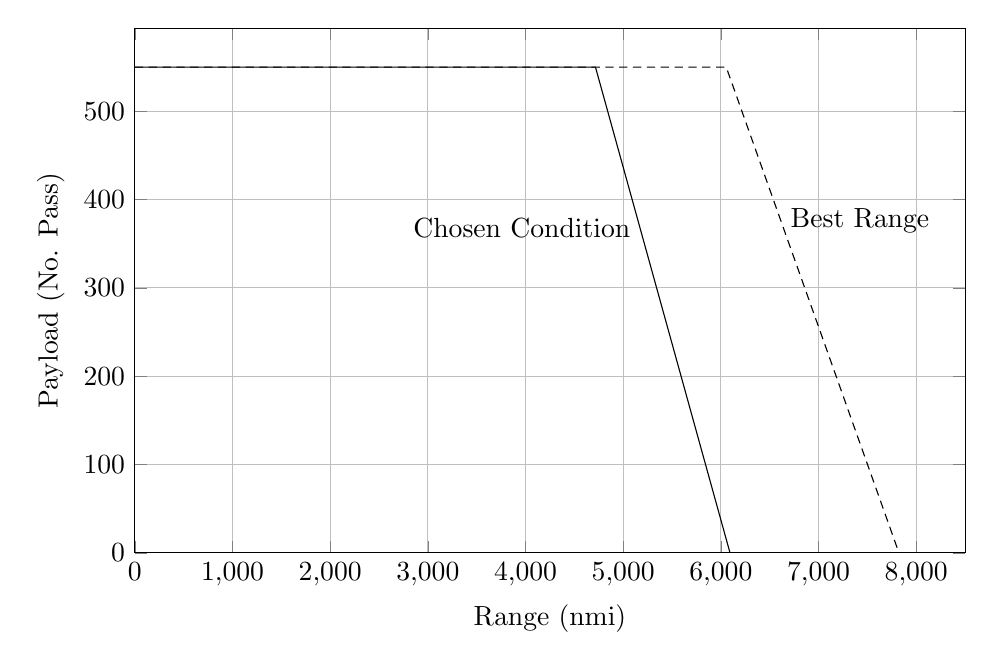
\begin{tikzpicture}

\begin{axis}[
%width=\figurewidth,
%height=\figureheight,
width=\textwidth,
height=0.68\textwidth,
scaled ticks=false, tick label style={/pgf/number format/fixed},
xmin=0.0,
xmax=8500,
xlabel={Range (nmi)},
xmajorgrids,
ymin=0.0,
ymax=594.0,
ylabel={Payload (No. Pass)},
ymajorgrids,
legend style={at={(1.03,0.5)},anchor=west,draw=black,fill=white,legend cell align=left}
]

\addplot [
color=black,
densely dashed
]
table[row sep=crcr]{
0.0	550.0\\
6052.69159914772	550.0\\
6054.4245495302075	550.0\\
7823.0998142333265	0.0\\
}node[right,pos=0.84] {Best Range};

\addplot [
color=black,
solid
]
table[row sep=crcr]{
0.0	550.0\\
4714.449641326871	550.0\\
4715.799438714584	550.0\\
6093.4229853161405	0.0\\
}node[left,pos=0.84] {Chosen Condition};
\end{axis}
\end{tikzpicture}%

\caption{B747-100B Payload-Range - Chosen Mach number and best range comparison}
\end{figure}
%
\begin{figure}[!b]
\centering
%PayloadRange_MaxTakeOffMass
\begin{tikzpicture}

\begin{axis}[
%width=\figurewidth,
%height=\figureheight,
width=\textwidth,
height=0.65\textwidth,
scaled ticks=false, tick label style={/pgf/number format/fixed},
/pgfplots/xtick={0,1000,...,7000},
xmin=0.0,
xmax=7205.947900774779,
xlabel={Range (nmi)},
xmajorgrids,
ymin=0.0,
ymax=594.0,
ylabel={Payload (No. Pass)},
ymajorgrids,
legend entries = {$\SI{284000}{\kilogram}$\\$\SI{302000}{\kilogram}$\\$\SI{319000}{\kilogram}$\\$\SI{337000}{\kilogram}$\\$\SI{355000}{\kilogram}$\\},
]

\addplot [
color=black,
dotted
]
table[row sep=crcr]{
0.0	550.0\\
2628.554546134139	550.0\\
7067.222791800295	-167.0\\
6454.2048688775485	0.0\\
};

\addplot [
color=black,
dashed 
]
table[row sep=crcr]{
0.0	550.0\\
3271.0963458251163	550.0\\
6414.600293103482	12.0\\
6454.2048688775485	0.0\\
};

\addplot [
color=black,
dashdotted
]
table[row sep=crcr]{
0.0	550.0\\
3876.900868736732	550.0\\
5866.414933662355	191.0\\
6454.2048688775485	0.0\\
};

\addplot [
color=black,
densely dashed
]
table[row sep=crcr]{
0.0	550.0\\
4449.942788313299	550.0\\
5398.867689125114	370.0\\
6454.2048688775485	0.0\\
};

\addplot [
color=black,
solid
]
table[row sep=crcr]{
0.0	550.0\\
4993.5847064047575	550.0\\
4995.014423148988	550.0\\
6454.2048688775485	0.0\\
};
\end{axis}
\end{tikzpicture}%

\caption{B747-100B Payload-Range - Maximum take-off mass parameterization}
\end{figure}